\section{Results}

\subsection{Ideal situation}
\label{sec:ideal_situation}
30 images and spectrums where run through the software and the average value was compared to each other. The spatial and spectral averages are plotted against each other in figure \ref{fig:spectral_vs_spatial_values} together with three linear regression lines, one for each color. 


\begin{figure}[h]
    \centering
    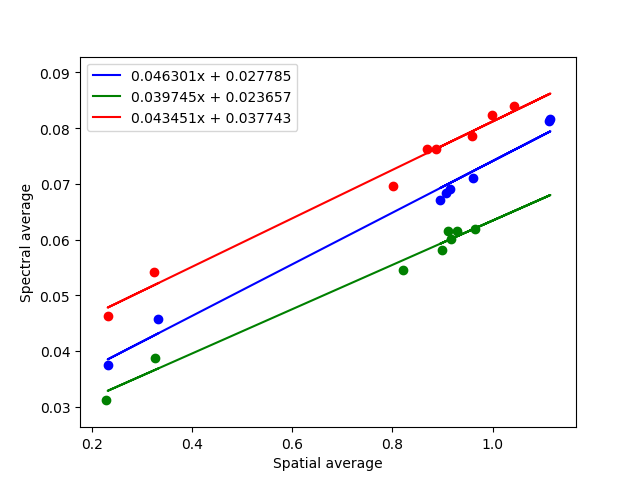
\includegraphics[width=0.75\textwidth]{Plots/spectral_vs_spatial_average_with_regression.png}
    \caption{Spatial and spectral averages plotted against each other with the fitted regression lines}
    \label{fig:spectral_vs_spatial_values}
\end{figure}

\subsection{Pertubation}
To see how well the value can be used for testing correspondence between image and spectrum, several images where taken that show non-ideal situations. These images will be compared to the regression lines created in section \ref{sec:ideal_situation} with the error function. These images are made with 10 randomly chosen settings from the ideal case, but with some unideal pertubation. 

For both the ideal and unideal cases the average error and variance of the error compared to the regression line was calculated and is presented in \ref{tb:error_estimate}.

\begin{table}[h]
    \centering
    \caption{Estimated error of the regression lines}
    \label{tb:error_estimate}
    \begin{tabular}{@{}llllllll@{}}
    \toprule
                   &                 & \multicolumn{3}{l}{Error average} & \multicolumn{3}{l}{Error variance} \\ \midrule
    Situation      & \#              & Blue       & Green     & Red      & Blue       & Green     & Red       \\
    Ideal          & 30              & 0.001261   & 0.001229  & 0.001370 & 6.744e-07  & 5.384e-07 & 8.963e-07 \\
    Ambient light  & 10              & 0.001805   & 0.001544  & 0.002349 & 1.860e-06  & 2.488e-06 & 1.016e-06 \\
    Border object  & 10              & 0.0007057  & 0.0005739 & 0.001615 & 6.581e-07  & 2.114e-07 & 6.382e-07 \\
    Outside object & 10              & 0.0006382  & 0.0009339 & 0.002476 & 1.174e-07  & 1.430e-07 & 1.876e-07 \\ \bottomrule
    \end{tabular}
\end{table}


\textbf{Ambient light}
These images where taken without turning of the light in the room. And with a fluorescent stand lamp on pointing towards the measurement area. Figure \ref{fig:ambient_light_plot} shows how these data points compare to the regression lines made in the ideal situation.

\begin{figure}[h]
    \centering
    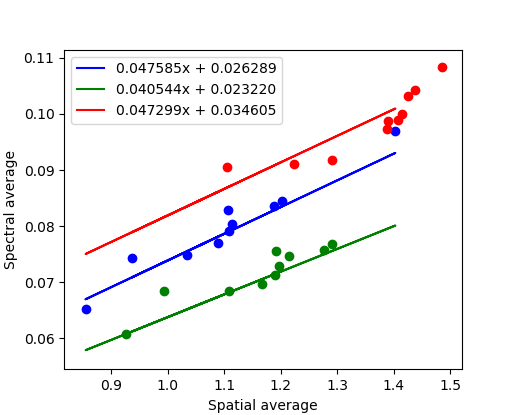
\includegraphics[width=0.5\textwidth]{Plots/spectral_vs_spatial_average_with_regression_ambient_light.png}
    \caption{Ambient light data points compared to ideal regression line}
    \label{fig:ambient_light_plot}
\end{figure}

\textbf{Border of imaging area}
Objects where put so that they where only partly inside the imaging area, but could still be seen by the spectrometer. Figure \ref{fig:boundary_objects_plot} shows how these data points compare to the regression lines made in the ideal situation.

\begin{figure}[h]
    \centering
    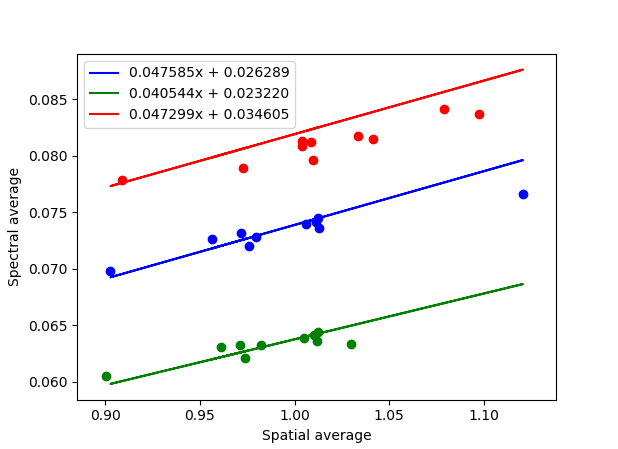
\includegraphics[width=0.5\textwidth]{Plots/spectral_vs_spatial_average_with_regression_boundary_objects.png}
    \caption{Objects placed on the boundary}
    \label{fig:boundary_objects_plot}
\end{figure}

\textbf{Outside the image area}
The same object where put inside the cameras viewpoint for every image, but a different object where put just outside it. It should still be inside the spectrometers view angle. Figure \ref{fig:outside_objects_plot} shows how these data points compare to the regression lines made in the ideal situation.

\begin{figure}[h]
    \centering
    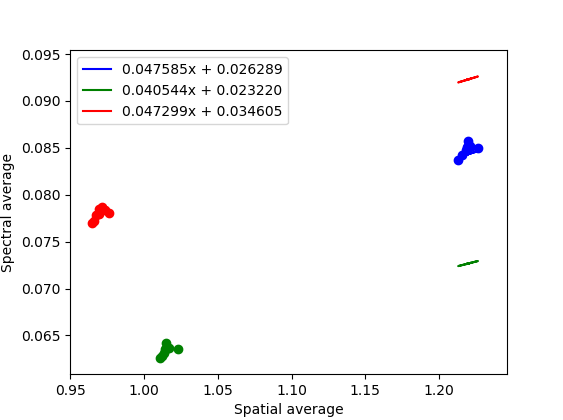
\includegraphics[width=0.5\textwidth]{Plots/spectral_vs_spatial_average_with_regression_outside_objects.png}
    \caption{One object inside boundary, another outside}
    \label{fig:outside_objects_plot}
\end{figure}

%\subsubsection{Specular reflection}

\section{Discussion}
The spatial and spectral average should be two sides of the same story, if the camera and the spectrometer are watching the same area and the conditions haven't changed between the camera taking the picture and the spectrometer taking the spectre. The purpose of taking these results where to test this postulate. 

Figure \ref{fig:spectral_vs_spatial_values} shows the results from 30 pictures taken under ideal conditions. The lines shown in blue, green and red are regression lines (sec \ref{sec:regression}) that are made as a minimum variance fit to the points. It looks like each of the color sensors have approximately the same number $a$, meaning that they have similar derivatives, but different $b$ means that they cross the y axis at different points. 

The error measurement given in table \ref{tb:error_estimate} shows the amount of error in the different situations. From the table we can see that the ambient light is the type of noise that is creating the most variance from the regression line. The other measurements actually show less variance which was not expected, but probably means that the acceptance cone of the spectrometer was smaller than expected, and not any bigger than the cameras acceptance cone. 

The effects of the dark current \ref{sec:noise_and_dark_current} was hopefully minimized by finding the relative reflectance and introducing the noise limit into the image processing. 